\documentclass[11pt]{article}
\usepackage{gensymb}
\usepackage{wasysym}
\usepackage{graphicx}
\usepackage[T1]{fontenc}
\usepackage[utf8]{inputenc}
\usepackage{polski}
\begin{document}
\textbf{Zginanie czyste}\\\\
Wymiary stanowiska pomiarowego\\
\begin{tabular}{|c|c|c|c|c|c|c|c|}
\hline
$l[mm]$ & $a[mm]$ & $E[MPa]$ & $b[mm]$ & $h[mm]$ & $A[mm^2]$ & $I_y[mm^4]$ & $W_Y[mm^3]$\\ \hline
1000 & $296$ & $2.1*10^5$ & $30$ & $20$ & $600$ & $2*10^4$ & $2*10^3$\\ \hline
\end{tabular}
\\\\\\
Wyniki pomiarów\\
\begin{tabular}{|c|c|c|c|c|c|c|}\hline
$lp.$ & $P[N]$ & $c_i[mm]$ & $f_c = c_i - c_0[mm]$ & $\epsilon_i[tens 8]$ & $\epsilon_i[tens 9]$ & $\epsilon_i[tens9] - \epsilon_0[tens9]$\\ \hline
0 & 0 & 7.5 & 0 & 0 & - 0.156 & 0\\ \hline
1 & 49.05 & 7.93 & 0.43 & 0.036 & -0.123 & 0.033\\ \hline
2 & 98.1 & 8.35 & 0.85 & 0.073 & -0.088 & 0.068\\ \hline
3 & 147.15 & 8.79 & 1.29 & 0.112 & -0.053 & 0.103\\ \hline
4 & 196.2 & 9.22 & 1.72 & 0.15 & -0.017 & 0.139\\ \hline
5 & 215.82 & 9.39 & 1.84 & 0.164 & -0.004 & 0.152\\ \hline
\end{tabular}
\\\\\\
Wyznaczanie doświadczalnej wartości modułu Younga na podstawie pomiaru czujnikowego\\
\begin{tabular}{cc}
Strzałka ugięcia: $f_c = \frac{Pal^2}{8EJ_y}$ & Błąd względny:\\\\
$E = \frac{Pal^2}{8J_yf_c}$ & $\frac{|E_i - E|}{E} * 100\%$\\\\
$E_1 = \frac{49.05 N * 0.296 m * 1^2 m}{8 * 2 * 10^-8 m^4 * 0.43 * 10^-3 m} \approx 211.029 GPa$ & $\frac{|211.029 GPa - 210 GPa|}{210 GPa} * 100\% = 0.49\%$\\\\
$E_2 = \frac{98.1 N * 0.296 m * 1^2 m}{8 * 2 * 10^-8 m^4 * 0.85 * 10^-3 m} \approx 213.512 GPa$ & $\frac{|213.512 GPa - 210 GPa|}{210 GPa} * 100\% \approx 1.67\%$\\\\
$E_3 = \frac{147.15 N * 0.296 m * 1^2 m}{8 * 2 * 10^-8 m^4 * 1.29 * 10^-3 m} \approx 211.029 GPa$ & $\frac{|211.029 GPa - 210 GPa|}{210 GPa} * 100\% = 0.49\%$\\\\
$E_4 = \frac{196.2 N * 0.296 m * 1^2 m}{8 * 2 * 10^-8 m^4 * 1.72 * 10^-3 m} \approx 211.029 GPa$ & $\frac{|211.029 GPa - 210 GPa|}{210 GPa} * 100\% = 0.49\%$\\\\
$E_5 = \frac{215.82 N * 0.296 m * 1^2 m}{8 * 2 * 10^-8 m^4 * 1.84 * 10^-3 m} \approx 216.993 GPa$ & $\frac{|216.993 GPa - 210 GPa|}{210 GPa} * 100\% = 3.33\%$\\
\end{tabular}
\\\\\\

2.3.2
Wyznaczanie doświadczalnej wartości modułu Younga na podstawie pomiaru tensometrycznego\\
$E = \frac{\sigma}{\epsilon} = \frac{M_gz}{I_y\epsilon} = \frac{Pah}{2I_y\epsilon}$\\
\begin{tabular}{cc}
Moduł Younga & Błąd względny\\
${E_1}_8 = \frac{49.05 N * 0.296 m * 2 * 10^{-2} m}{2 * 2 * 10^{-8} m^4 * 0.036 * 10^{-3}} \approx $ & $\frac{|198.888-210|}{210} * 100\% \approx 5.29\%$\\\\
${E_2}_8 = \frac{98.1 N * 0.296 m * 2 * 10^-2 m}{2 * 2 * 10^-8 m^4 * 0.036 * 10^{-3}} \approx 198.888 MPa$& $\frac{|198.888-210|}{210} * 100\% \approx 5.29\%$\\\\
${E_3}_8 = \frac{147.15 N * 0.296 m * 2 * 10^-2 m}{2 * 2 * 10^-8 m^4 * 0.036 * 10^{-3}} \approx $ & $\frac{|198.888-210|}{210} * 100\% \approx 5.29\%$\\\\
${E_4}_8 = \frac{196.2 N * 0.296 m * 2 * 10^-2 m}{2 * 2 * 10^-8 m^4 * 0.036 * 10^{-3}} \approx $ & $\frac{|198.888-210|}{210} * 100\% \approx 5.29\%$\\\\
${E_5}_8 = \frac{215.82 N * 0.296 m * 2 * 10^{-2} m}{2 * 2 * 10^{-8} m^4 * 0.036 * 10^{-3}} \approx $ 194.764 MPa & $\frac{|194.764-210|}{210} * 100\% \approx 7.26\%$\\
\end{tabular}\\\\

2.3.3
Wyznaczyć wartość doświadczalną krzywizny osi belki na podstawie pomiaru:\\
\textbf{a) czujnikowego:}\\
Korzystając z: $f_c = \frac{Pal^2}{8EJ_y}$\\
${f_c}_1 =\frac{215.82*0.296*1}{8*210*10^6*2*10^{-8}m^4}=0.0036m=3.6mm$\\\\
${f_c}_2 =\frac{98.1*0.296*1}{8*210*10^6*2*10^{-8}m^4}=0.00864m=0.8646mm$\\\\
${f_c}_3 =\frac{215.82*0.296*1}{8*210*10^6*2*10^{-8}m^4}=0.0036m=3.6mm$\\\\
${f_c}_4 =\frac{215.82*0.296*1}{8*210*10^6*2*10^{-8}m^4}=0.0036m=3.6mm$\\\\
${f_c}_5 =\frac{215.82*0.296*1}{8*210*10^6*2*10^{-8}m^4}=0.0036m=3.6mm$\\

\textbf{b) tensometrycznego} dla wskazanego obciążenia wraz z porównaniem z wielkością teoretyczną(wraz z błędem względnym):\\






\textbf{Zginanie poprzeczne}\\\\
\begin{tabular}{|c|c|c|c|c|c|c|}\hline
$P[N]$ & $c_{1i}$ & $c_{2i}$ & $\epsilon_i(13)$ & $\epsilon_i(14)$ & $\epsilon_i(15)$ & $\epsilon_i(16)$\\ \hline
$P_0 = 0$ & 0.25 & 7.1 & 0 & -0.72 & -0.139 & -0.118\\ \hline
$P_1 = 20$ & 3.4 & 5.65 & 0.023 & -0.687 & -0.129 & -0.086\\ \hline
$P_2 = 50$ & 5.13 & 3 & 0.075 & -0.621 & -0.106 & -0.028\\ \hline
$P_1 + P_2 = 70$ & 8.45 & 1.6 & 0.098 & -0.588 & -0.095 & 0.003\\ \hline
\end{tabular}\\\\
\\
\begin{tabular}{|c|c|c|c|c|c|c|}\hline
$P[N]$ & $c'_{1i}$ & $c'_{2i}$ & $\epsilon_i(13)$ & $\epsilon'_i(14)$ & $\epsilon'_i(15)$ & $\epsilon'_i(16)$\\ \hline
$P_0 = 0$ & 0 & 0 & 0 & 0 & 0 & 0\\ \hline
$P_1 = 20$ & 3.15 & 1.45 & 0.023 & 0.033 & 0.01 & 0.032\\ \hline
$P_2 = 50$ & 4.88 & 4.1 & 0.075 & 0.099 & 0.033 & 0.09\\ \hline
$P_1 + P_2 = 70$ & 8.2 & 5.5 & 0.098 & 0.132 & 0.044 & 0.121\\ \hline

\end{tabular}\\\\
Zasada superpozycji - suma przemieszczeń z pierwszego i drugiego obciążenia osobno jest przemieszczeniem dla sumy obciążeń:\\\\
\begin{tabular}{c|c|c}
dla $c'_1$: & 3.15 mm + 4.88 mm = 8.03 mm & $\frac{|8.2 mm - 8.03 mm|}{8.02 mm} * 100\% = 2.1\%$\\
dla $c'_2$: & 1.45 mm + 4.1 mm = 5.55 mm & $\frac{|5.5 mm - 5.55 mm|}{5.5 mm} * 100\% = 0.9\%$\\
dla $epsilon'(13)$: & 0.023 + 0.075 = 0.98 & $\frac{|0.98 - 0.98|}{0.98} * 100\% = 0\%$\\
dla $epsilon'(14)$: & 0.033 + 0.099 = 0.132 & $\frac{|0.132 - 0.132|}{0.132} * 100\% = 0\%$\\
dla $epsilon'(15)$: & 0.01 + 0.033= 0.043 & $\frac{|0.044 - 0.043|}{0.044} * 100\% = 2.3\%$\\
dla $epsilon'(16)$: & 0.032+ 0.09 = 0.122 & $\frac{|0.121 - 0.122|}{0.121} * 100\% = 0.8\%$\\
\end{tabular}\\\\
Powyższe wyniki, z powodu niskich błędów względnych (mniej niż $3\%$), można uznać za wiarygodne sprawdzenie zasady superpozycji na przykładzie zginanej belki.\\

Zasada Bettiego - praca wykonana przez pierwsze obciążenie na przemieszczeniu wywołanym drugim obciążeniem jest równa pracy drugiego obciążenia na przemieszczeniu wywołanym przez pierwsze:\\
$P1 * c_{12} = P2 * c_{21}$\\
20 N * 4.88 mm = 50 N * 1.45 mm\\
97.6 N * mm $\approx$ 72.5 N * mm\\
W przypadku zasady Bettiego wyniki doświadczalne odbiegają od założeń teoretycznych. Przyczyną tego mogą być nieliniowości w badanym ustroju.\\\\


\textbf{Zginanie ukośne}\\\\
\begin{tabular}{|c|c|c|c|c|c|}\hline
$ $ & $V_i[N]$ & $\epsilon_i(1)$ & $\epsilon_i(2)$ & $\epsilon_i(3)$ & $\epsilon_i(4)$ \\ \hline
0 & 0 & 0 & -0.077 & -0.299 & -0.257 \\ \hline
1 & 50 & 0.277 & -0.16 & -0.377 & -0.16 \\ \hline
2 & 70 & 0.39 & -0.195 & -0.41 & -0.13 \\ \hline
\end{tabular}\\\\
\begin{tabular}{|c|c|c|c|c|c|}\hline
$ $ & $V_i[N]$ & $\epsilon_i(1)$ & $\epsilon'_i(2)$ & $\epsilon'_i(3)$ & $\epsilon'_i(4)$ \\ \hline
0 & 0 & 0 & 0 & 0 & 0 \\ \hline
1 & 50 & 0.277 & -0.083 & -0.078 & 0.097 \\ \hline
2 & 70 & 0.39 & -0.118 & -0.111 & 0.127 \\ \hline
\end{tabular}\\\\
dural - E = 73 GPa\\
Wartości doświadczalne naprężeń ($\sigma = |\epsilon * E|$):\\
$\sigma_1 = 0.277\permil * 73 GPa = 20.221 MPa$\\
$\sigma_2 = -0.083\permil * 73 GPa = -6.059 MPa$\\
$\sigma_3 = -0.078\permil * 73 GPa = -5.694 MPa$\\
$\sigma_4 = 0.097\permil * 73 GPa = 7.081 MPa$\\
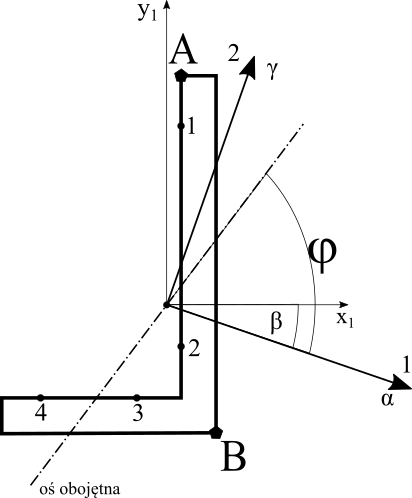
\includegraphics{path7520-7.png}\\
Współrzędne środka ciężkości:\\
$x_c = \frac{30 mm * 5 mm * 15 mm + 45 mm * 5 mm * 27.5 mm}{30 mm * 5 mm + 45 mm * 5 mm} = 22.5 mm$\\
$y_c = \frac{30 mm * 5 mm * 2.5 mm + 45 mm * 5 mm * 27.5 mm}{30 mm * 5 mm + 45 mm * 5 mm} = 17.5 mm$\\
$S_c = [22.5 mm; 17.5 mm]$\\
Momenty bezwładności względem osi $x_1$ i $ y_1$:\\
$I_{x_1} = \frac{5 mm * (45 mm)^3}{12} + 5 mm * 43 mm * (27.5 mm - 17.5 mm)^2 + \frac{30 mm * (5 mm)^3}{12} + 5 mm * 30 mm * (17.5 mm - 2.5 mm)^2 = 59468.75 mm^4 + 34062.5 mm^4 = 93531.25 mm^4$\\
$I_{y_1} = \frac{5 mm * (30 mm)^3}{12} + 5 mm * 30 mm * (22.5 mm - 15 mm)^2 + \frac{45 mm * (5 mm)^3}{12} + 45 mm * 5 mm * (27.5 mm - 22.5 mm)^2 = 19687.5 mm^4 + 6093.75 mm^4 = 25781.25 mm^4$\\
Moment dewiacyjny względem układu $x_1y_1$:\\
$I_{x_1y_1} = 0 + (22.5 mm - 15 mm) * (17.5 mm - 2.5 mm) * 30 mm * 5 mm + 0 + (27.5 mm - 22.5 mm) * (27.5 mm - 17.5 mm) * 45 mm * 5 mm = 28125 mm^4$\\
Momenty główne bezwładności:\\
$I = \frac{I_{x_1} + I_{y_1}}{2} \pm \sqrt{\left(\frac{I_{x_1} + I_{y_1}}{2}\right)^2 + I_{x_1y_1}^2}$\\
$I_1 = \frac{93531.25 mm^4 + 25781 mm^4}{2} + \sqrt{\left(\frac{93531.25 mm^4 + 25781.25 mm^4}{2}\right)^2 + (28125 mm^4)^2} = 107562.78 mm^4$\\
$I_2 = \frac{93531.25 mm^4 + 25781 mm^4}{2} - \sqrt{\left(\frac{93531.25 mm^4 + 25781.25 mm^4}{2}\right)^2 + (28125 mm^4)^2} = 11749.22 mm^4$\\
Kąt orientacji układu z osiami głównymi względem układu $x_1y_1$:\\
$tg(2\beta) = \frac{-2I_{x_1y_1}}{I_{x_1} - I_{y_1}}$\\
$tg(2\beta) = \frac{-2 * 28125 mm^4}{93531.25 mm^4 - 25781 mm^4} = -0.830255$\\
$\beta = -19.9\degree \approx -20\degree$\\
Wektor momentu gnącego zrzutowany na osie nowego układu:\\
$M_\alpha = M * cos\beta = 50 N * 1 m * cos20\degree = 47 Nm$\\
$M_\gamma = M * sin\beta = 50 N * 1 m * sin20\degree = 17.1 Nm$\\
Równanie funkcji naprężeń:\\
$\sigma = \frac{M_\gamma}{I_2}\alpha - \frac{M_\alpha}{I_1}\gamma$\\
$\sigma = \frac{17.1 Nm}{11749.22 mm^4}\alpha - \frac{47 Nm}{107562.78 mm^4}\gamma$\\
$\sigma = 1455443016\alpha - 436957289\gamma [\frac{N}{m^3}]$\\
Szukamy osi obojętnej:\\
$\sigma = 0   \Rightarrow   0 = 1455443016\alpha - 436957289\gamma$\\
$\gamma = 3,330858\alpha$  -  równanie osi obojętnej w układzie osi głównych\\
$\phi \approx 73.3\degree$ - kąt o jaki obrócona jest oś obojętna\\
\\
Transformacja współrzędnych z układu pierwotnego do układu osi głównych:\\
$\alpha = x_1cos\beta - y_1sin\beta$\\
$\gamma = x_1sin\beta + y_1cos\beta$\\
Punkt A($x_1,y_1$) = [2.5 mm, 32.5 mm]:\\
$\alpha_A = 2.5 mm * cos(20\degree) - 32.5 mm * sin(20\degree) \approx -8.77 mm$\\
$\gamma_A = 2.5 mm * sin(20\degree) + 32.5 mm * cos(20\degree) \approx 31.4 mm$\\
Punkt B($x_1,y_1$) = [7.5 mm, -17.5 mm]:\\
$\alpha_B = 7.5 mm * cos(20\degree) + 17.5 mm * sin(20\degree) \approx 13.03 mm$\\
$\gamma_B = 7.5 mm * sin(20\degree) - 17.5 mm * cos(20\degree)
\approx -13.88 mm$\\
\\
Naprężenia w A:\\
$\sigma_A = 1455443016 \frac{N}{m^3} * (-8.77) mm - 436957289 \frac{N}{m^3} * 31.4 mm = -26.485 MPa$\\
Naprężenia w B:\\
$\sigma_B = 1455443016 \frac{N}{m^3} * 13.03 mm - 436957289 \frac{N}{m^3} * (-13.88) mm = 25.029 MPa$\\
\\
W naprężeniach należy uwzględnić, że faktyczne znaki są różne od powyższych, co zaznaczono na wykresie naprężeń.\\
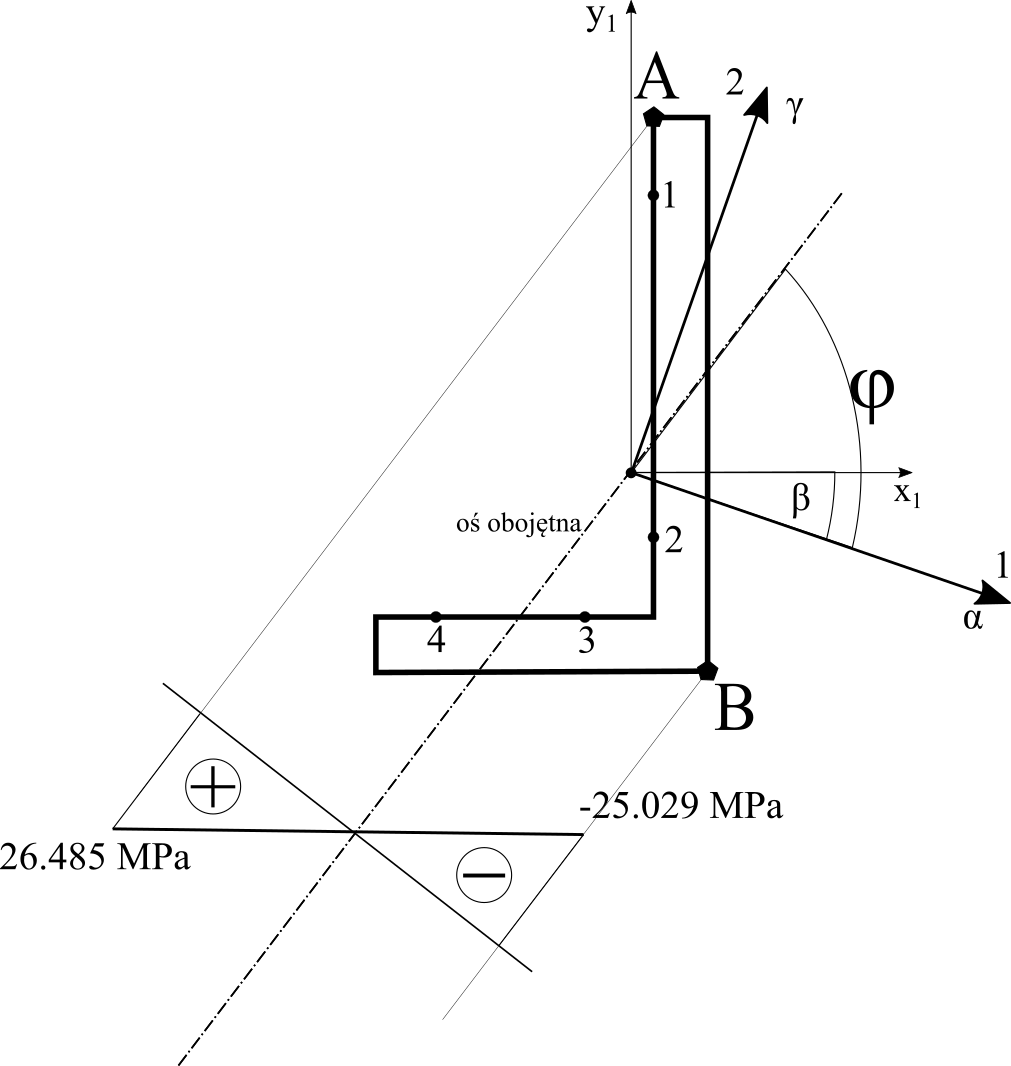
\includegraphics{wykres.png}\\
Współrzędne tensometrów w układzie $x_1y_1$:\\
\begin{tabular}{c|c|c}
tensometr & $x_1[mm]$ & $y_1[mm]$\\ \hline
1 & 2.5 & 25.5\\
2 & 2.5 & -5.3\\
3 & -3.7, & -12.5\\	
4 & -17.1 & -12.5\\
\end{tabular}\\
\\
Transformacja do układu osi głównych $\alpha\gamma$:\\
\begin{tabular}{c|c|c}
tensometr & $\alpha[mm]$ & $\gamma[mm]$\\ \hline
1 & -6.37 & 24.82\\
2 & 4.16 & -4.13\\
3 & 0.8, & -13.01\\
4 & -11.79 & -17.59\\
\end{tabular}
\\
\begin{tabular}{c|c}
tensometr & naprężenie [MPa]\\ \hline
1 & -20.116\\
2 & 7.859\\
3 & 6.849\\
4 & -9.474\\
\end{tabular}
\\
Błąd względny pomiarów tensometrycznych naprężeń:\\
\begin{tabular}{cc}
tensometr & błąd względny\\
1 & $\frac{||-20.116 MPa|-|20.221 MPa||}{|-20.116 MPa|} * 100\% \approx 0.52\%$\\
2 & $\frac{||7.859 MPa|-|6.059 MPa||}{|7.859 MPa|} * 100\% \approx 22.9\%$\\
3 & $\frac{||6.849 MPa|-|5.694 MPa||}{|6.849 MPa|} * 100\% \approx 16.9\%$\\
4 & $\frac{||-9.474 MPa|-|7.081 MPa||}{|-9.474 MPa|} * 100\% \approx 25.3\%$\\
\end{tabular}\\
\\\\\\
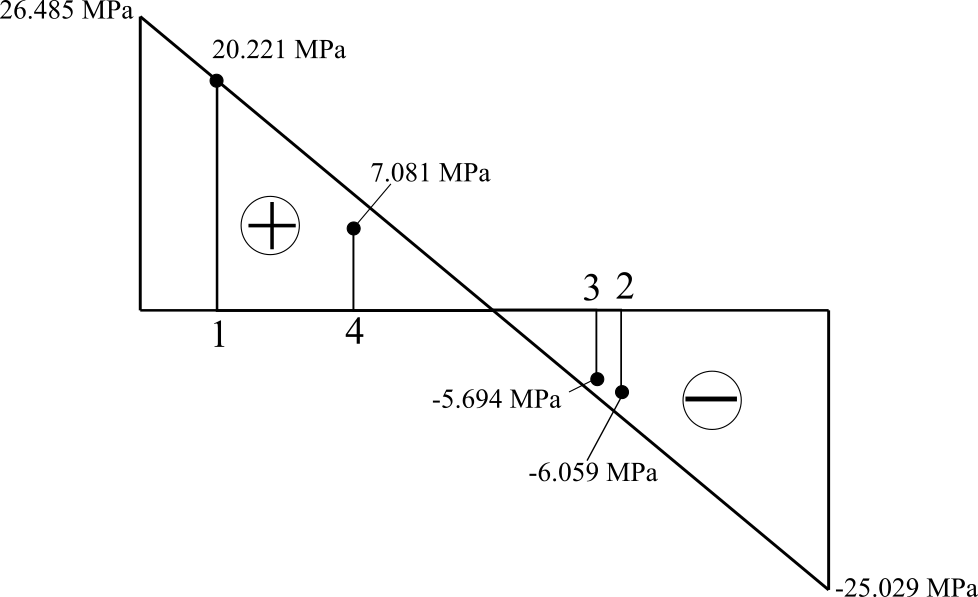
\includegraphics{wykres_diff.png}








\end{document}